\chapter{El problema del matrimonio estable} \label{me}
%\begin{flushright}
%\textit{``Even the worst husband, God forbid, is better than no husband, God forbid.''}
%\end{flushright}
En el pequeño Shtetl\footnote{Poblado en Yddish.} de Anatevka, había muchos hombres y muchas mujeres jóvenes con el deseo de casarse. Yenta, la casamentera del pueblo, tenía el trabajo y la obligación de emparejar a todos estos jóvenes. Esta tarea sonará fácil pero no lo es, cada joven tenía distintas preferencias y cada uno de ellos necesitaba un trato especial, ``el matrimonio es para toda la vida y no es algo que hay que tomar como si fuera cualquier cosa" decía Yenta. Retomando los conceptos de la última sección, se desea que el emparejamiento de estos jóvenes sea estable y óptimo si es que es posible.\footnote{Este problema hace el supuesto de que las relaciones solo pueden ser entre un hombre y una mujer y que esto es reflejado por sus preferencias. Esto no manifiesta la realidad o las opiniones del autor y se hace únicamente con fines matemáticos.}
En términos matemáticos, supongamos que tenemos $n$ hombres $\alpha_1,\alpha_2,\ldots,\alpha_n$ y $m$ mujeres $a_1, a_2,\ldots,a_m$ con las restricciones:
\begin{enumerate}
\item \begin{equation} \label{1r1}
x_{i,j}= 
\begin{cases}
1 & \qquad \text{si $i$ se casa con $j$.} \\
0 &\qquad\text{en otro caso.}\ \\ 
\end{cases} \end{equation}
\item \begin{equation} \label{1r2}
\sum_{j=1}^{m}x_{i,j} \leq1 \ \text{ para toda $i=1,2,\ldots,n$. }
\end{equation} Cada hombre se casa con a lo más una mujer. 
\item \begin{equation} \label{1r3}
\sum_{i=1}^{n} x_{i,j} \leq 1\ \text{ para toda $j=1,2,\dots,m$.} 
\end{equation}
Cada mujer se casa con a lo más un hombre. 
\end{enumerate}

Es claro, a partir de la definición del problema que éste es un caso particular del problema original. Aprovechando lo que se hizo en la sección anterior la definición de la matriz de preferencias, un emparejamiento estable y de un emparejamiento óptimo son análogas a las definiciones \ref{matpref}, \ref{Estable} y \ref{optima}. Existen diversos resultados sobre el problema del matrimonio estable, uno de los más famosos es por Gale y Shapley que encontraron un algoritmo que siempre encuentra un emparejamiento estable y además lo hace sin muchas complicaciones. 

Un supuesto adicional que haremos es que el número de hombres es exactamente igual al número de mujeres. Esto se verá después que es relativamente sencillo de generalizar al caso en el que el número de hombres y de mujeres no es igual. 

%Definición del problema
%Definiciones alternativas
%

%Ejemplos

\section{Algoritmo de Gale Shapley}
En 1962 David Gale y Lloyd Stowell Shapley demostraron que para el problema del matrimonio estable siempre se puede encontrar un emparejamiento estable óptimo para los hombres, esto se hizo enunciando un algoritmo y mostrando su convergencia. El algoritmo queda representado por el siguiente código y es conocido como el algoritmo de Gale Shapley.

%\begin{lstlisting}[style=R, escapeinside={(*}{*)},caption={Algoritmo de Gale Shapley}, captionpos=b, label=c1]
%Input : Una matriz de preferencias para (*$n$*) hombres y (*$n$*) mujeres 
%Output: Un emparejamiento. 
%Cada hombre le propone a la primera mujer de su lista. Cada mujer que recibe más de una propuesta acepta la que este más arriba en su lista y rechaza al resto. 
%repeat{ #hasta que todos los hombres tengan pareja
%Los hombres no emparejados le proponen a la siguiente mujer en su lista. 
%Cada mujer que recibe una propuesta escoge la que está más arriba en su lista entre las propuestas que recibió y su pareja actual.
%Las mujeres rechazan las propuestas que no aceptaron.
%}
%\end{lstlisting}

\IncMargin{1em}
\begin{Algoritmo}[H]
%\SetKwData{Left}{left}\SetKwData{This}{this}\SetKwData{Up}{up}
%\SetKwFunction{Union}{Union}\SetKwFunction{FindCompress}{FindCompress}
\SetKwInOut{Input}{input}\SetKwInOut{Output}{output}
\Input{Una matriz de preferencias para $n$ hombres y $n$ mujeres}
\Output{Un emparejamiento. }
\BlankLine
\emph{Cada hombre le propone a la primera mujer de su lista\; Cada mujer que recibe más de una propuesta acepta la que este más arriba en su lista y rechaza al resto \; }
\Repeat{hasta que todos los hombres tengan pareja}{
	\emph{Los hombres no emparejados le proponen a la siguiente mujer en su lista\; } 
	\emph{Cada mujer que recibe una propuesta escoge la que está más arriba en su lista entre las propuestas que recibió y su pareja actual\;} 
	\emph{Las mujeres rechazan las propuestas que no aceptaron\;} 
}
\caption{Gale Shapley}
\end{Algoritmo}
\DecMargin{1em}
Para dejar la explicación un poco más clara es importante mostrar un ejemplo de cómo funciona el algoritmo y cuál es su resultado final.
\begin{eje}{\cite{GaleShapley}}
\label{ejemploGS}
Supongamos que para 4 hombres y 4 mujeres tenemos la matriz de preferencias 
$$\begin{pmatrix}
& A & B & C & D \\
\alpha & 1,3 & 2,2 & 3,1 & 4,3 \\
\beta & 1,4 & 2,3 & 3,2 & 4,4 \\
\gamma & 3,1 & 1,4 & 2,3 & 4,2 \\
\delta & 2,2&3,1 &1,4 & 4,1 
\end{pmatrix}.$$
En la primera iteración, $\alpha$ le propone matrimonio a $A$, $\beta$ le propone matrimonio a $A$, $\gamma$ le propone matrimonio a $B$ y $\delta$ le propone matrimonio a $C$.

\begin{figure}[H]\centering

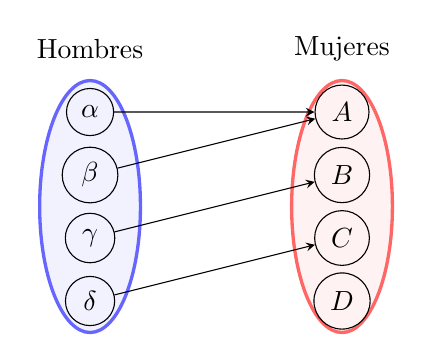
\begin{tikzpicture}[ scale=0.8]
\tikzset{vertex/.style = {shape=circle,draw,minimum size=1.5em}}
\tikzset{edge/.style = {->,> = latex}}
\filldraw[color=blue!60, fill=blue!5, very thick](0,2.5) ellipse (.8 and 2);
\filldraw[color=red!60, fill=red!5, very thick](4,2.5) ellipse (.8 and 2);


% vertices
% 


\node[vertex] (a) at (0,4) {$\alpha$};
\node[vertex] (b) at (0,3) {$\beta$};
\node[vertex] (c) at (0,2) {$\gamma$};
\node[vertex] (d) at (0,1) {$\delta$};

\node[vertex] (e) at (4,4) {$A$};
\node[vertex] (f) at (4,3) {$B$};
\node[vertex] (g) at (4,2) {$C$};
\node [vertex] (h) at (4,1) {$D$};

\node (i) at (0,5) {Hombres};
\node (j) at (4,5) {Mujeres};

\path[-stealth] (a) edge (e);
\path[-stealth] (b) edge (e);
\path[-stealth] (c) edge (f);
\path[-stealth] (d) edge (g);



%\draw (0.2,8)--(3.8,8);



\end{tikzpicture}

\caption{Primera iteración.}
\end{figure}

En la segunda iteración, $A$ acepta la propuesta de $\alpha$ y $\beta$ le propone matrimonio a $B$.

\begin{figure}[H]
\centering

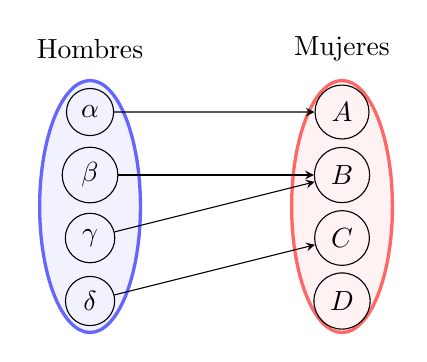
\begin{tikzpicture}[ scale=0.8]
\tikzset{vertex/.style = {shape=circle,draw,minimum size=1.5em}}
\tikzset{edge/.style = {->,> = latex}}
\filldraw[color=blue!60, fill=blue!5, very thick](0,2.5) ellipse (.8 and 2);
\filldraw[color=red!60, fill=red!5, very thick](4,2.5) ellipse (.8 and 2);


% vertices
% 


\node[vertex] (a) at (0,4) {$\alpha$};
\node[vertex] (b) at (0,3) {$\beta$};
\node[vertex] (c) at (0,2) {$\gamma$};
\node[vertex] (d) at (0,1) {$\delta$};

\node[vertex] (e) at (4,4) {$A$};
\node[vertex] (f) at (4,3) {$B$};
\node[vertex] (g) at (4,2) {$C$};
\node [vertex] (h) at (4,1) {$D$};

%\draw (0,.5) node[cross,red] {};

\node (i) at (0,5) {Hombres};
\node (j) at (4,5) {Mujeres};

\path[-stealth] (a) edge (e);
\path[-stealth] (b) edge (f);
\path[-stealth] (c) edge (f);
\path[-stealth] (d) edge (g);



%\draw (0.2,8)--(3.8,8);



\end{tikzpicture}

\caption{Segunda iteración.}
\end{figure}


En la tercera iteración, $B$ acepta la propuesta de $\beta$ y $\gamma$ le propone matrimonio a $C$.

\begin{figure}[H]\centering

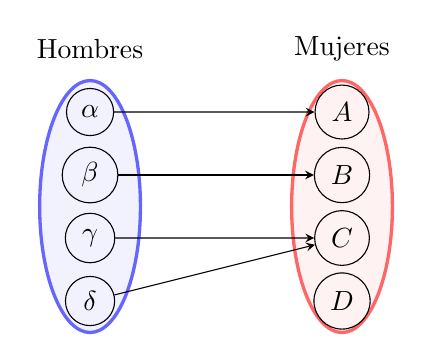
\begin{tikzpicture}[ scale=0.8]
\tikzset{vertex/.style = {shape=circle,draw,minimum size=1.5em}}
\tikzset{edge/.style = {->,> = latex}}
\filldraw[color=blue!60, fill=blue!5, very thick](0,2.5) ellipse (.8 and 2);
\filldraw[color=red!60, fill=red!5, very thick](4,2.5) ellipse (.8 and 2);


% vertices
% 


\node[vertex] (a) at (0,4) {$\alpha$};
\node[vertex] (b) at (0,3) {$\beta$};
\node[vertex] (c) at (0,2) {$\gamma$};
\node[vertex] (d) at (0,1) {$\delta$};

\node[vertex] (e) at (4,4) {$A$};
\node[vertex] (f) at (4,3) {$B$};
\node[vertex] (g) at (4,2) {$C$};
\node [vertex] (h) at (4,1) {$D$};

\node (i) at (0,5) {Hombres};
\node (j) at (4,5) {Mujeres};

\path[-stealth] (a) edge (e);
\path[-stealth] (b) edge (f);
\path[-stealth] (c) edge (g);
\path[-stealth] (d) edge (g);



%\draw (0.2,8)--(3.8,8);



\end{tikzpicture}

\caption{Tercera iteración.}
\end{figure}

En la cuarta iteración, $C$ acepta la propuesta de $\gamma$ y $\delta$ le propone matrimonio a $A$.

\begin{figure}[H]\centering

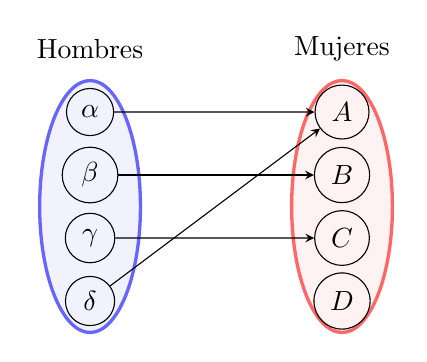
\begin{tikzpicture}[ scale=0.8]
\tikzset{vertex/.style = {shape=circle,draw,minimum size=1.5em}}
\tikzset{edge/.style = {->,> = latex}}
\filldraw[color=blue!60, fill=blue!5, very thick](0,2.5) ellipse (.8 and 2);
\filldraw[color=red!60, fill=red!5, very thick](4,2.5) ellipse (.8 and 2);


% vertices
% 


\node[vertex] (a) at (0,4) {$\alpha$};
\node[vertex] (b) at (0,3) {$\beta$};
\node[vertex] (c) at (0,2) {$\gamma$};
\node[vertex] (d) at (0,1) {$\delta$};

\node[vertex] (e) at (4,4) {$A$};
\node[vertex] (f) at (4,3) {$B$};
\node[vertex] (g) at (4,2) {$C$};
\node [vertex] (h) at (4,1) {$D$};

\node (i) at (0,5) {Hombres};
\node (j) at (4,5) {Mujeres};

\path[-stealth] (a) edge (e);
\path[-stealth] (b) edge (f);
\path[-stealth] (c) edge (g);
\path[-stealth] (d) edge (e);



%\draw (0.2,8)--(3.8,8);



\end{tikzpicture}

\caption{Cuarta iteración.}
\end{figure}


En la quinta iteración, $A$ acepta la propuesta de $\delta$ y $\alpha$ le propone matrimonio a $B$.

\begin{figure}[H]\centering

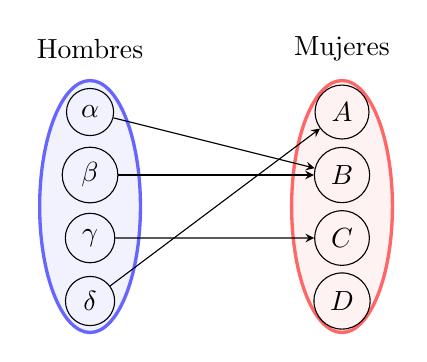
\begin{tikzpicture}[ scale=0.8]
\tikzset{vertex/.style = {shape=circle,draw,minimum size=1.5em}}
\tikzset{edge/.style = {->,> = latex}}
\filldraw[color=blue!60, fill=blue!5, very thick](0,2.5) ellipse (.8 and 2);
\filldraw[color=red!60, fill=red!5, very thick](4,2.5) ellipse (.8 and 2);


% vertices
% 


\node[vertex] (a) at (0,4) {$\alpha$};
\node[vertex] (b) at (0,3) {$\beta$};
\node[vertex] (c) at (0,2) {$\gamma$};
\node[vertex] (d) at (0,1) {$\delta$};

\node[vertex] (e) at (4,4) {$A$};
\node[vertex] (f) at (4,3) {$B$};
\node[vertex] (g) at (4,2) {$C$};
\node [vertex] (h) at (4,1) {$D$};

\node (i) at (0,5) {Hombres};
\node (j) at (4,5) {Mujeres};

\path[-stealth] (a) edge (f);
\path[-stealth] (b) edge (f);
\path[-stealth] (c) edge (g);
\path[-stealth] (d) edge (e);



%\draw (0.2,8)--(3.8,8);



\end{tikzpicture}

\caption{Quinta iteración.}
\end{figure}

En la sexta iteración, $B$ acepta la propuesta de $\alpha$ y $\beta$ le propone matrimonio a $C$.

\begin{figure}[H]\centering

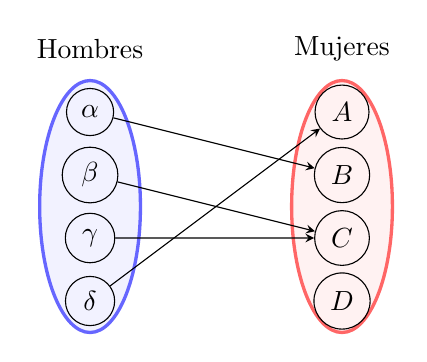
\begin{tikzpicture}[ scale=0.8]
\tikzset{vertex/.style = {shape=circle,draw,minimum size=1.5em}}
\tikzset{edge/.style = {->,> = latex}}
\filldraw[color=blue!60, fill=blue!5, very thick](0,2.5) ellipse (.8 and 2);
\filldraw[color=red!60, fill=red!5, very thick](4,2.5) ellipse (.8 and 2);


% vertices
% 


\node[vertex] (a) at (0,4) {$\alpha$};
\node[vertex] (b) at (0,3) {$\beta$};
\node[vertex] (c) at (0,2) {$\gamma$};
\node[vertex] (d) at (0,1) {$\delta$};

\node[vertex] (e) at (4,4) {$A$};
\node[vertex] (f) at (4,3) {$B$};
\node[vertex] (g) at (4,2) {$C$};
\node [vertex] (h) at (4,1) {$D$};

\node (i) at (0,5) {Hombres};
\node (j) at (4,5) {Mujeres};

\path[-stealth] (a) edge (f);
\path[-stealth] (b) edge (g);
\path[-stealth] (c) edge (g);
\path[-stealth] (d) edge (e);



%\draw (0.2,8)--(3.8,8);



\end{tikzpicture}

\caption{Sexta iteración.}
\end{figure}

En la séptima iteración, $C$ acepta la propuesta de $\beta$ y $\gamma$ le propone matrimonio a $A$.

\begin{figure}[H]\centering

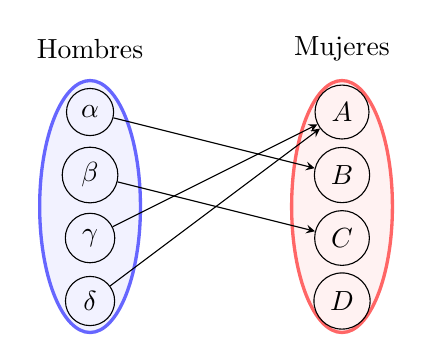
\begin{tikzpicture}[ scale=0.8]
\tikzset{vertex/.style = {shape=circle,draw,minimum size=1.5em}}
\tikzset{edge/.style = {->,> = latex}}
\filldraw[color=blue!60, fill=blue!5, very thick](0,2.5) ellipse (.8 and 2);
\filldraw[color=red!60, fill=red!5, very thick](4,2.5) ellipse (.8 and 2);


% vertices
% 


\node[vertex] (a) at (0,4) {$\alpha$};
\node[vertex] (b) at (0,3) {$\beta$};
\node[vertex] (c) at (0,2) {$\gamma$};
\node[vertex] (d) at (0,1) {$\delta$};

\node[vertex] (e) at (4,4) {$A$};
\node[vertex] (f) at (4,3) {$B$};
\node[vertex] (g) at (4,2) {$C$};
\node [vertex] (h) at (4,1) {$D$};

\node (i) at (0,5) {Hombres};
\node (j) at (4,5) {Mujeres};

\path[-stealth] (a) edge (f);
\path[-stealth] (b) edge (g);
\path[-stealth] (c) edge (e);
\path[-stealth] (d) edge (e);



%\draw (0.2,8)--(3.8,8);



\end{tikzpicture}

\caption{Séptima iteración.}
\end{figure}


En la octava iteración, $A$ acepta la propuesta de $\gamma$ y $\delta$ le propone matrimonio a $B$.

\begin{figure}[H]\centering

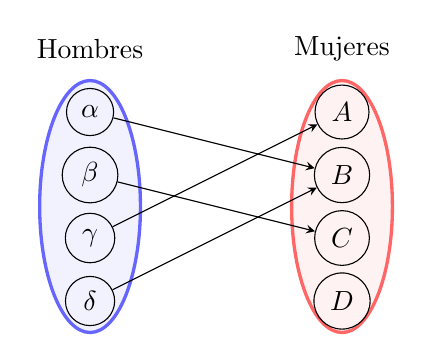
\begin{tikzpicture}[ scale=0.8]
\tikzset{vertex/.style = {shape=circle,draw,minimum size=1.5em}}
\tikzset{edge/.style = {->,> = latex}}
\filldraw[color=blue!60, fill=blue!5, very thick](0,2.5) ellipse (.8 and 2);
\filldraw[color=red!60, fill=red!5, very thick](4,2.5) ellipse (.8 and 2);


% vertices
% 


\node[vertex] (a) at (0,4) {$\alpha$};
\node[vertex] (b) at (0,3) {$\beta$};
\node[vertex] (c) at (0,2) {$\gamma$};
\node[vertex] (d) at (0,1) {$\delta$};

\node[vertex] (e) at (4,4) {$A$};
\node[vertex] (f) at (4,3) {$B$};
\node[vertex] (g) at (4,2) {$C$};
\node [vertex] (h) at (4,1) {$D$};

\node (i) at (0,5) {Hombres};
\node (j) at (4,5) {Mujeres};

\path[-stealth] (a) edge (f);
\path[-stealth] (b) edge (g);
\path[-stealth] (c) edge (e);
\path[-stealth] (d) edge (f);



%\draw (0.2,8)--(3.8,8);



\end{tikzpicture}

\caption{Octava iteración.}
\end{figure}

En la novena iteración, $B$ acepta la propuesta de $\delta$ y $\alpha$ le propone matrimonio a $C$.

\begin{figure}[H]\centering

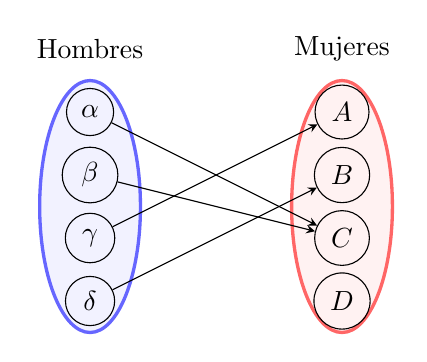
\begin{tikzpicture}[ scale=0.8]
\tikzset{vertex/.style = {shape=circle,draw,minimum size=1.5em}}
\tikzset{edge/.style = {->,> = latex}}
\filldraw[color=blue!60, fill=blue!5, very thick](0,2.5) ellipse (.8 and 2);
\filldraw[color=red!60, fill=red!5, very thick](4,2.5) ellipse (.8 and 2);


% vertices
% 


\node[vertex] (a) at (0,4) {$\alpha$};
\node[vertex] (b) at (0,3) {$\beta$};
\node[vertex] (c) at (0,2) {$\gamma$};
\node[vertex] (d) at (0,1) {$\delta$};

\node[vertex] (e) at (4,4) {$A$};
\node[vertex] (f) at (4,3) {$B$};
\node[vertex] (g) at (4,2) {$C$};
\node [vertex] (h) at (4,1) {$D$};

\node (i) at (0,5) {Hombres};
\node (j) at (4,5) {Mujeres};

\path[-stealth] (a) edge (g);
\path[-stealth] (b) edge (g);
\path[-stealth] (c) edge (e);
\path[-stealth] (d) edge (f);



%\draw (0.2,8)--(3.8,8);



\end{tikzpicture}

\caption{Novena iteración.}
\end{figure}


En la décima iteración, $C$ acepta la propuesta de $\alpha$, $\beta$ le propone matrimonio a $D$ y $D$ acepta la propuesta de $\beta$. Después de 10 pasos en el algoritmo, todos los hombres ya están emparejados, es decir, el algoritmo convergió en un emparejamiento. Cabe mencionar que el número total de propuestas fue 13. 

\begin{figure}[H]\centering

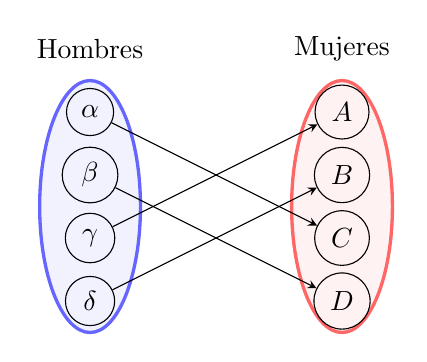
\begin{tikzpicture}[ scale=0.8]
\tikzset{vertex/.style = {shape=circle,draw,minimum size=1.5em}}
\tikzset{edge/.style = {->,> = latex}}
\filldraw[color=blue!60, fill=blue!5, very thick](0,2.5) ellipse (.8 and 2);
\filldraw[color=red!60, fill=red!5, very thick](4,2.5) ellipse (.8 and 2);


% vertices
% 


\node[vertex] (a) at (0,4) {$\alpha$};
\node[vertex] (b) at (0,3) {$\beta$};
\node[vertex] (c) at (0,2) {$\gamma$};
\node[vertex] (d) at (0,1) {$\delta$};

\node[vertex] (e) at (4,4) {$A$};
\node[vertex] (f) at (4,3) {$B$};
\node[vertex] (g) at (4,2) {$C$};
\node [vertex] (h) at (4,1) {$D$};

\node (i) at (0,5) {Hombres};
\node (j) at (4,5) {Mujeres};

\path[-stealth] (a) edge (g);
\path[-stealth] (b) edge (h);
\path[-stealth] (c) edge (e);
\path[-stealth] (d) edge (f);



%\draw (0.2,8)--(3.8,8);



\end{tikzpicture}

\caption{Décima iteración.}
\end{figure}
\fin
\end{eje}

Lo importante de este algoritmo no es solo que produce un emparejamiento, adicional a esto como lo muestra el siguiente teorema, el emparejamiento resultante es estable. 
\begin{teo}[Teorema de Gale Shaley] \cite{GaleShapley} \\
\label{teorema de Gale Shapley}
El algoritmo de Gale Shapley termina en un emparejamiento estable.
\end{teo}
\begin{proof}
Supongamos que el emparejamiento producido por el algoritmo no es estable. Esto es, un hombre $\alpha$ y una mujer $A$ se prefieren entre ellos que a sus respectivas parejas. 

Como $\alpha$ prefiere a $A$ más que a su esposa entonces, $\alpha$ le propuso matrimonio primero a $A$ que a su propia esposa. 
Además, como $A$ prefiere a $\alpha$ sobre su esposo entonces, $A$ hubiera rechazado a su esposo y se hubiera quedado casada con $\alpha$ lo cual es una contradicción. 

Por lo tanto, el algoritmo de Gale Shapley termina siempre en un emparejamiento estable. 
\end{proof}
Un resultado inmediato de esto es que siempre, sin importar como sean las preferencias, existe un emparejamiento estable. 
\begin{cor}
\label{corexiste}
Dada una matriz de preferencias arbitraria existe un emparejamiento estable. 
\end{cor}
\begin{proof}
Si aplicamos el algoritmo de Gale Shapley, sabemos por el teorema \ref{teorema de Gale Shapley} que este siempre acaba en un emparejamiento estable. Por lo tanto, siempre existe un emparejamiento estable.
\end{proof}

Una vez que sabemos que el algoritmo siempre converge, nos interesa conocer que tan rápido lo hace y si tiene algunas ventajas el emparejamiento resultante. El lema \ref{lema 1} nos ayuda a llegar a estos resultados y los corolarios \ref{cor1} y \ref{cor2} nos dan una idea de qué tan bueno es el algoritmo. 
\begin{lem} 
\label{lema 1} \cite{Knuth} \\
Bajo el emparejamiento obtenido por Gale Shapley, solo un hombre puede terminar con la última mujer de su lista como pareja. 
\end{lem}

\begin{proof}

Supongamos que en el emparejamiento de Gale Shapley $m$ ($m\geq2$) hombres terminan con la última mujer de su lista como pareja, eso significa que cada uno de esos $m$ hombres invitó a salir a todas las mujeres. Entonces cada mujer fue invita a salir por lo menos $m$ veces, lo cual es una contradicción porque el algoritmo acaba cuando invitan a salir a la última mujer y a ésta solo la invitan a salir una vez. Por lo tanto, solo un hombre puede terminar con la última mujer de su lista como pareja. 
\end{proof}

Dos consecuencias casi inmediatas de esto son que bajo el algoritmo la gran mayoría de los hombres no terminan con su última opción y que el algoritmo converge relativamente rápido. 
\begin{cor}
\label{cor1}
Si en un emparejamiento estable por lo menos dos hombres están emparejados con la última mujer de sus respectivas listas, entonces existen dos o más emparejamientos estables en el problema.
\end{cor}

\begin{proof}
Llamemos $M$ al emparejamiento estable donde por lo menos dos hombres están emparejados con la última mujer de sus respectivas listas y llamemos $M'$ al emparejamiento de Gale Shapley.
Por el teorema \ref{teorema de Gale Shapley} sabemos que el algoritmo de Gale Shapley siempre acaba en un emparejamiento estable y además en ese emparejamiento estable solo un hombre puede terminar con la última mujer de su lista como pareja por el lema \ref{lema 1}.
Por lo tanto $m$ y $m'$ son diferentes y como ambos son emparejamientos estables entonces el número de emparejamientos estables en el problema es mayor o igual a dos. 
\end{proof}

\begin{cor}
\label{cor2}
El número máximo de propuestas en el algoritmo es $n^2-n+1$
\end{cor}

\begin{proof}
Por el lema \ref{lema 1} sabemos que a lo más un hombre acaba emparejado con la última mujer de su lista, por lo tanto, el peor emparejamiento posible para el algoritmo es uno donde $n-1$ hombres terminan con la penúltima mujer de sus respectivas listas y un hombre termina con la última. Para llegar a esta situación de acuerdo con el algoritmo, los $n-1$ hombres deben de realizar $n-1$ propuestas cada uno y el otro hombre debe de realizar $n$ propuestas. Esto es $(n-1)(n-1)+n$ propuestas que es igual a $n^2-n+1$ propuestas.
\end{proof}

\begin{obs}
\label{complejidad1}
La complejidad del algoritmo de Gale Shapley es del orden de $n^2$.
\end{obs}

\begin{eje}
Si retomamos el ejemplo \ref{ejemploGS} podemos ver que para 4 personas hubo $4^{2}-4+1=13$ propuestas que es el máximo número posible de éstas de acuerdo con el corolario \ref{cor2}.
\fin
\end{eje}

A partir de esto ya podemos resolver el problema en el que la cantidad de hombres y de mujeres es distinta. El siguiente resultado muestra que sin importar el número de hombres o de mujeres, el algoritmo también converge. 

\begin{teo} \cite{GaleShapley} \\
Dada una matriz de preferencias arbitraria con $n$ hombres y $m$ mujeres, el algoritmo de Gale Shapley converge a un emparejamiento estable
\end{teo}
\begin{proof}
Supongamos que la cantidad de hombres es más chica que la cantidad de mujeres ($n<m$), en este caso el algoritmo acaba cuando $n$ de las $m$ mujeres reciben una propuesta. Si suponemos que la cantidad de hombres es mayor a la cantidad de mujeres ($n>m$), en este caso el algoritmo acaba después de que $n-m$ hombres son rechazados por todas las mujeres y las propuestas de $m$ de los hombres son aceptadas. 

Además de forma análoga al teorema \ref{teorema de Gale Shapley} se puede ver que el emparejamiento producido es estable.
\end{proof}
A partir de esto podemos generalizar el algoritmo de Gale Shapley para que permita un número distinto de hombres y de mujeres. 

\IncMargin{1em}
\begin{Algoritmo}[H]
%\SetKwData{Left}{left}\SetKwData{This}{this}\SetKwData{Up}{up}
%\SetKwFunction{Union}{Union}\SetKwFunction{FindCompress}{FindCompress}
\SetKwInOut{Input}{input}\SetKwInOut{Output}{output}
\Input{Una matriz de preferencias para $n$ hombres y $m$ mujeres}
\Output{Un emparejamiento. }
\BlankLine
\emph{Cada hombre le propone a la primera mujer de su lista\; Cada mujer que recibe más de una propuesta acepta la que esté más arriba en su lista y rechaza al resto \; }
\Repeat{hasta que todos los hombres tengan pareja o hasta que sean rechazados por todas las mujeres}{
	\emph{Los hombres no emparejados le proponen a la siguiente mujer en su lista\; } 
	\emph{Cada mujer que recibe una propuesta escoge la que está más arriba en su lista entre las propuestas que recibió y su pareja actual\;} 
	\emph{Las mujeres rechazan las propuestas que no aceptaron\;} 
}
\caption{Gale Shapley para un número distinto de hombres y mujeres}
\end{Algoritmo}
\DecMargin{1em}


El algoritmo de Gale Shapley no es el único algoritmo que existe para producir un emparejamiento estable, y si se cambia el algoritmo el emparejamiento producido podría ser totalmente diferente al producido por el primero. De forma inmediata se puede crear un algoritmo igual al de Gale Shapley con la única diferencia de que las mujeres les proponen a los hombres, esto está representado por el siguiente código.


%\begin{lstlisting}[style=R, escapeinside={(*}{*)},caption={Algoritmo de Gale Shapley para las mujeres}, captionpos=b, label=c1]
%Input : Una matriz de preferencias para (*$n$*) hombres y (*$n$*) mujeres 
%Output: Un emparejamiento. 
%Cada mujer le propone al primer hombre de su lista. Cada hombre que recibe más de una propuesta acepta la que este más arriba en su lista y rechaza al resto. 
%repeat{ #hasta que todas las mujeres tengan pareja
%Los hombres no emparejados le proponen al siguiente hombre en su lista. 
%Cada hombre que recibe una propuesta escoge la que está más arriba en su lista entre las propuestas que recibió y su pareja actual.
%Los hombres rechazan las propuestas que no aceptaron.
%}
%\end{lstlisting}

\IncMargin{1em}
\begin{Algoritmo}[H]
%\SetKwData{Left}{left}\SetKwData{This}{this}\SetKwData{Up}{up}
%\SetKwFunction{Union}{Union}\SetKwFunction{FindCompress}{FindCompress}
\SetKwInOut{Input}{input}\SetKwInOut{Output}{output}

\Input{Una matriz de preferencias para $n$ hombres y $m$ mujeres }
\Output{Un emparejamiento.}
\BlankLine
\emph{Cada mujer le propone al primer hombre de su lista\; Cada hombre que recibe más de una propuesta acepta la que este más arriba en su lista y rechaza al resto\; }
\Repeat{hasta que todas las mujeres tengan pareja o o hasta que sean rechazadas por todas los hombres}{
	\emph{Las mujeres no emparejadas le proponen al siguiente hombre en su lista\; } 
	\emph{Cada hombre que recibe una propuesta escoge la que está más arriba en su lista entre las propuestas que recibió y su pareja actual\;} 
	\emph{Los hombres rechazan las propuestas que no aceptaron\;} 
}
\caption{Gale Shapley para las mujeres}
\end{Algoritmo}
\DecMargin{1em}


El siguiente ejemplo ilustra que el emparejamiento obtenido es distinto en ciertas situaciones y que por lo tanto los emparejamientos estables no son únicos. 

\begin{eje}
\label{ejeunico}
Retomando el ejemplo \ref{ejemplo matrimonio 1}. \\
Si aplicamos el algoritmo de Gale Shapley para los hombres obtenemos en primera estancia el siguiente emparejamiento estable. 
\begin{figure}[H]\centering

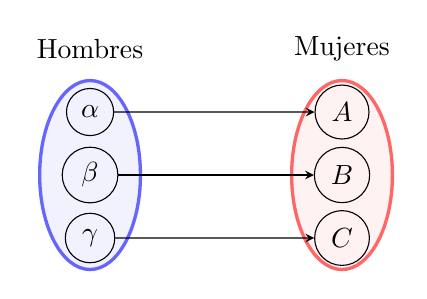
\begin{tikzpicture}[ scale=0.8]
\tikzset{vertex/.style = {shape=circle,draw,minimum size=1.5em}}
\tikzset{edge/.style = {->,> = latex}}
\filldraw[color=blue!60, fill=blue!5, very thick](0,3) ellipse (.8 and 1.5);
\filldraw[color=red!60, fill=red!5, very thick](4,3) ellipse (.8 and 1.5);


% vertices
% 


\node[vertex] (a) at (0,4) {$\alpha$};
\node[vertex] (b) at (0,3) {$\beta$};
\node[vertex] (c) at (0,2) {$\gamma$};


\node[vertex] (e) at (4,4) {$A$};
\node[vertex] (f) at (4,3) {$B$};
\node[vertex] (g) at (4,2) {$C$};


\node (i) at (0,5) {Hombres};
\node (j) at (4,5) {Mujeres};

\path[-stealth] (a) edge (e);
\path[-stealth] (b) edge (f);
\path[-stealth] (c) edge (g);



%\draw (0.2,8)--(3.8,8);



\end{tikzpicture}

\caption{Resultado del algoritmo si los hombres proponen.}
\end{figure}

Si aplicamos el algoritmo de Gale Shapley para las mujeres obtenemos en primera estancia el siguiente emparejamiento estable. 
\begin{figure}[H]\centering

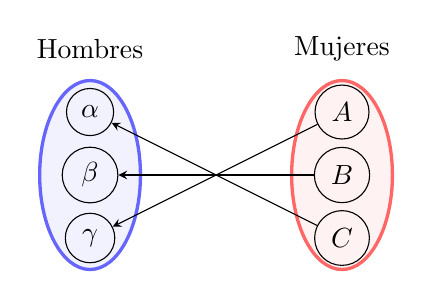
\begin{tikzpicture}[ scale=0.8]
\tikzset{vertex/.style = {shape=circle,draw,minimum size=1.5em}}
\tikzset{edge/.style = {->,> = latex}}
\filldraw[color=blue!60, fill=blue!5, very thick](0,3) ellipse (.8 and 1.5);
\filldraw[color=red!60, fill=red!5, very thick](4,3) ellipse (.8 and 1.5);


% vertices
% 


\node[vertex] (a) at (0,4) {$\alpha$};
\node[vertex] (b) at (0,3) {$\beta$};
\node[vertex] (c) at (0,2) {$\gamma$};


\node[vertex] (e) at (4,4) {$A$};
\node[vertex] (f) at (4,3) {$B$};
\node[vertex] (g) at (4,2) {$C$};


\node (i) at (0,5) {Hombres};
\node (j) at (4,5) {Mujeres};

\path[-stealth] (g) edge (a);
\path[-stealth] (f) edge (b);
\path[-stealth] (e) edge (c);



%\draw (0.2,8)--(3.8,8);



\end{tikzpicture}

\caption{Resultado del algoritmo si las mujeres proponen.}
\end{figure}

Es fácil ver que los dos emparejamientos estables son distintos.
\fin
\end{eje}

\begin{cor}
Dada una matriz de preferencias arbitraria, la cantidad de emparejamientos estables es mayor o igual a 1. 
\end{cor}
\begin{proof}
Con el corolario \ref{corexiste} podemos garantizar la existencia y con el ejemplo \ref{ejeunico} mostramos que no podemos garantizar la unicidad de éste.
\end{proof}


Para continuar, podemos generalizar el problema del matrimonio estable a uno que permite a los hombres casarse con varias mujeres cambiando su cota superior de uno a cualquier otro número. Este es conocido como el problema de admisión a universidades. 
